%
%  progress-presentation.tex
%  src
%
%  Created by Illya Starikov on 09/16/17.
%  Copyright 2017. Illya Starikov. All rights reserved.
%

% \documentclass[notes,xcolor=dvipsnames]{beamer}       % print frame + notes
% \documentclass[notes=only,xcolor=dvipsnames]{beamer}  % only notes
\documentclass[xclolor=dvipsnames]{beamer}            % only frames
%\documentclass[handout,xclolor=dvipsnames]{beamer}    % only frames, no pauses
\usepackage{soul,graphics}

\usepackage{amssymb,amsmath,verbatim,graphicx,microtype,upquote,units,booktabs,akkwidepage}

\newcommand{\chapterNumber}[1]{
    \setcounter{section}{#1}
    \addtocounter{section}{-1}
}
\title{Vim (Presentation \#4)}
\subtitle{Special Topics (CS3001)}
\author{Illya Starikov}
\date{Sometimes In The Future}
\institute{Missouri University of Science and Technology}

\usepackage[export]{adjustbox}

\begin{document}
\begin{darkframes}
    \maketitle

    \begin{frame}
        \frametitle{A Brief Introduction}

        They often say

        \begin{quote}
            ``A Developer Is Only As Good As His Tools''
        \end{quote}

        Although I don't agree with this sentiment, I always wanted to become better with tools I was constantly using. One of the tools I use most is my code editor: \href{https://www.vim.org}{Vim}.

    \end{frame}

    \begin{frame}
        \frametitle{A Brief Introduction}

        \begin{itemize}
            \item Vim has been around since 1991, and is almost ubiquitous on all Unix machines. It has served mostly as a terminal text editor (see attached video).
            \item Also, Vim has greatly improved a lot since then, to incorporate many of the new features that IDEs and Text Editors have brought to the table.
            \item Along with that, a lot of projects have set out to make Vim look and feel more like a regular text editor (as apposed to a terminal editor).
        \end{itemize}
    \end{frame}

    \begin{frame}[fragile]
        \frametitle{A Brief Introduction}
        \begin{figure}[H]
            \centering
            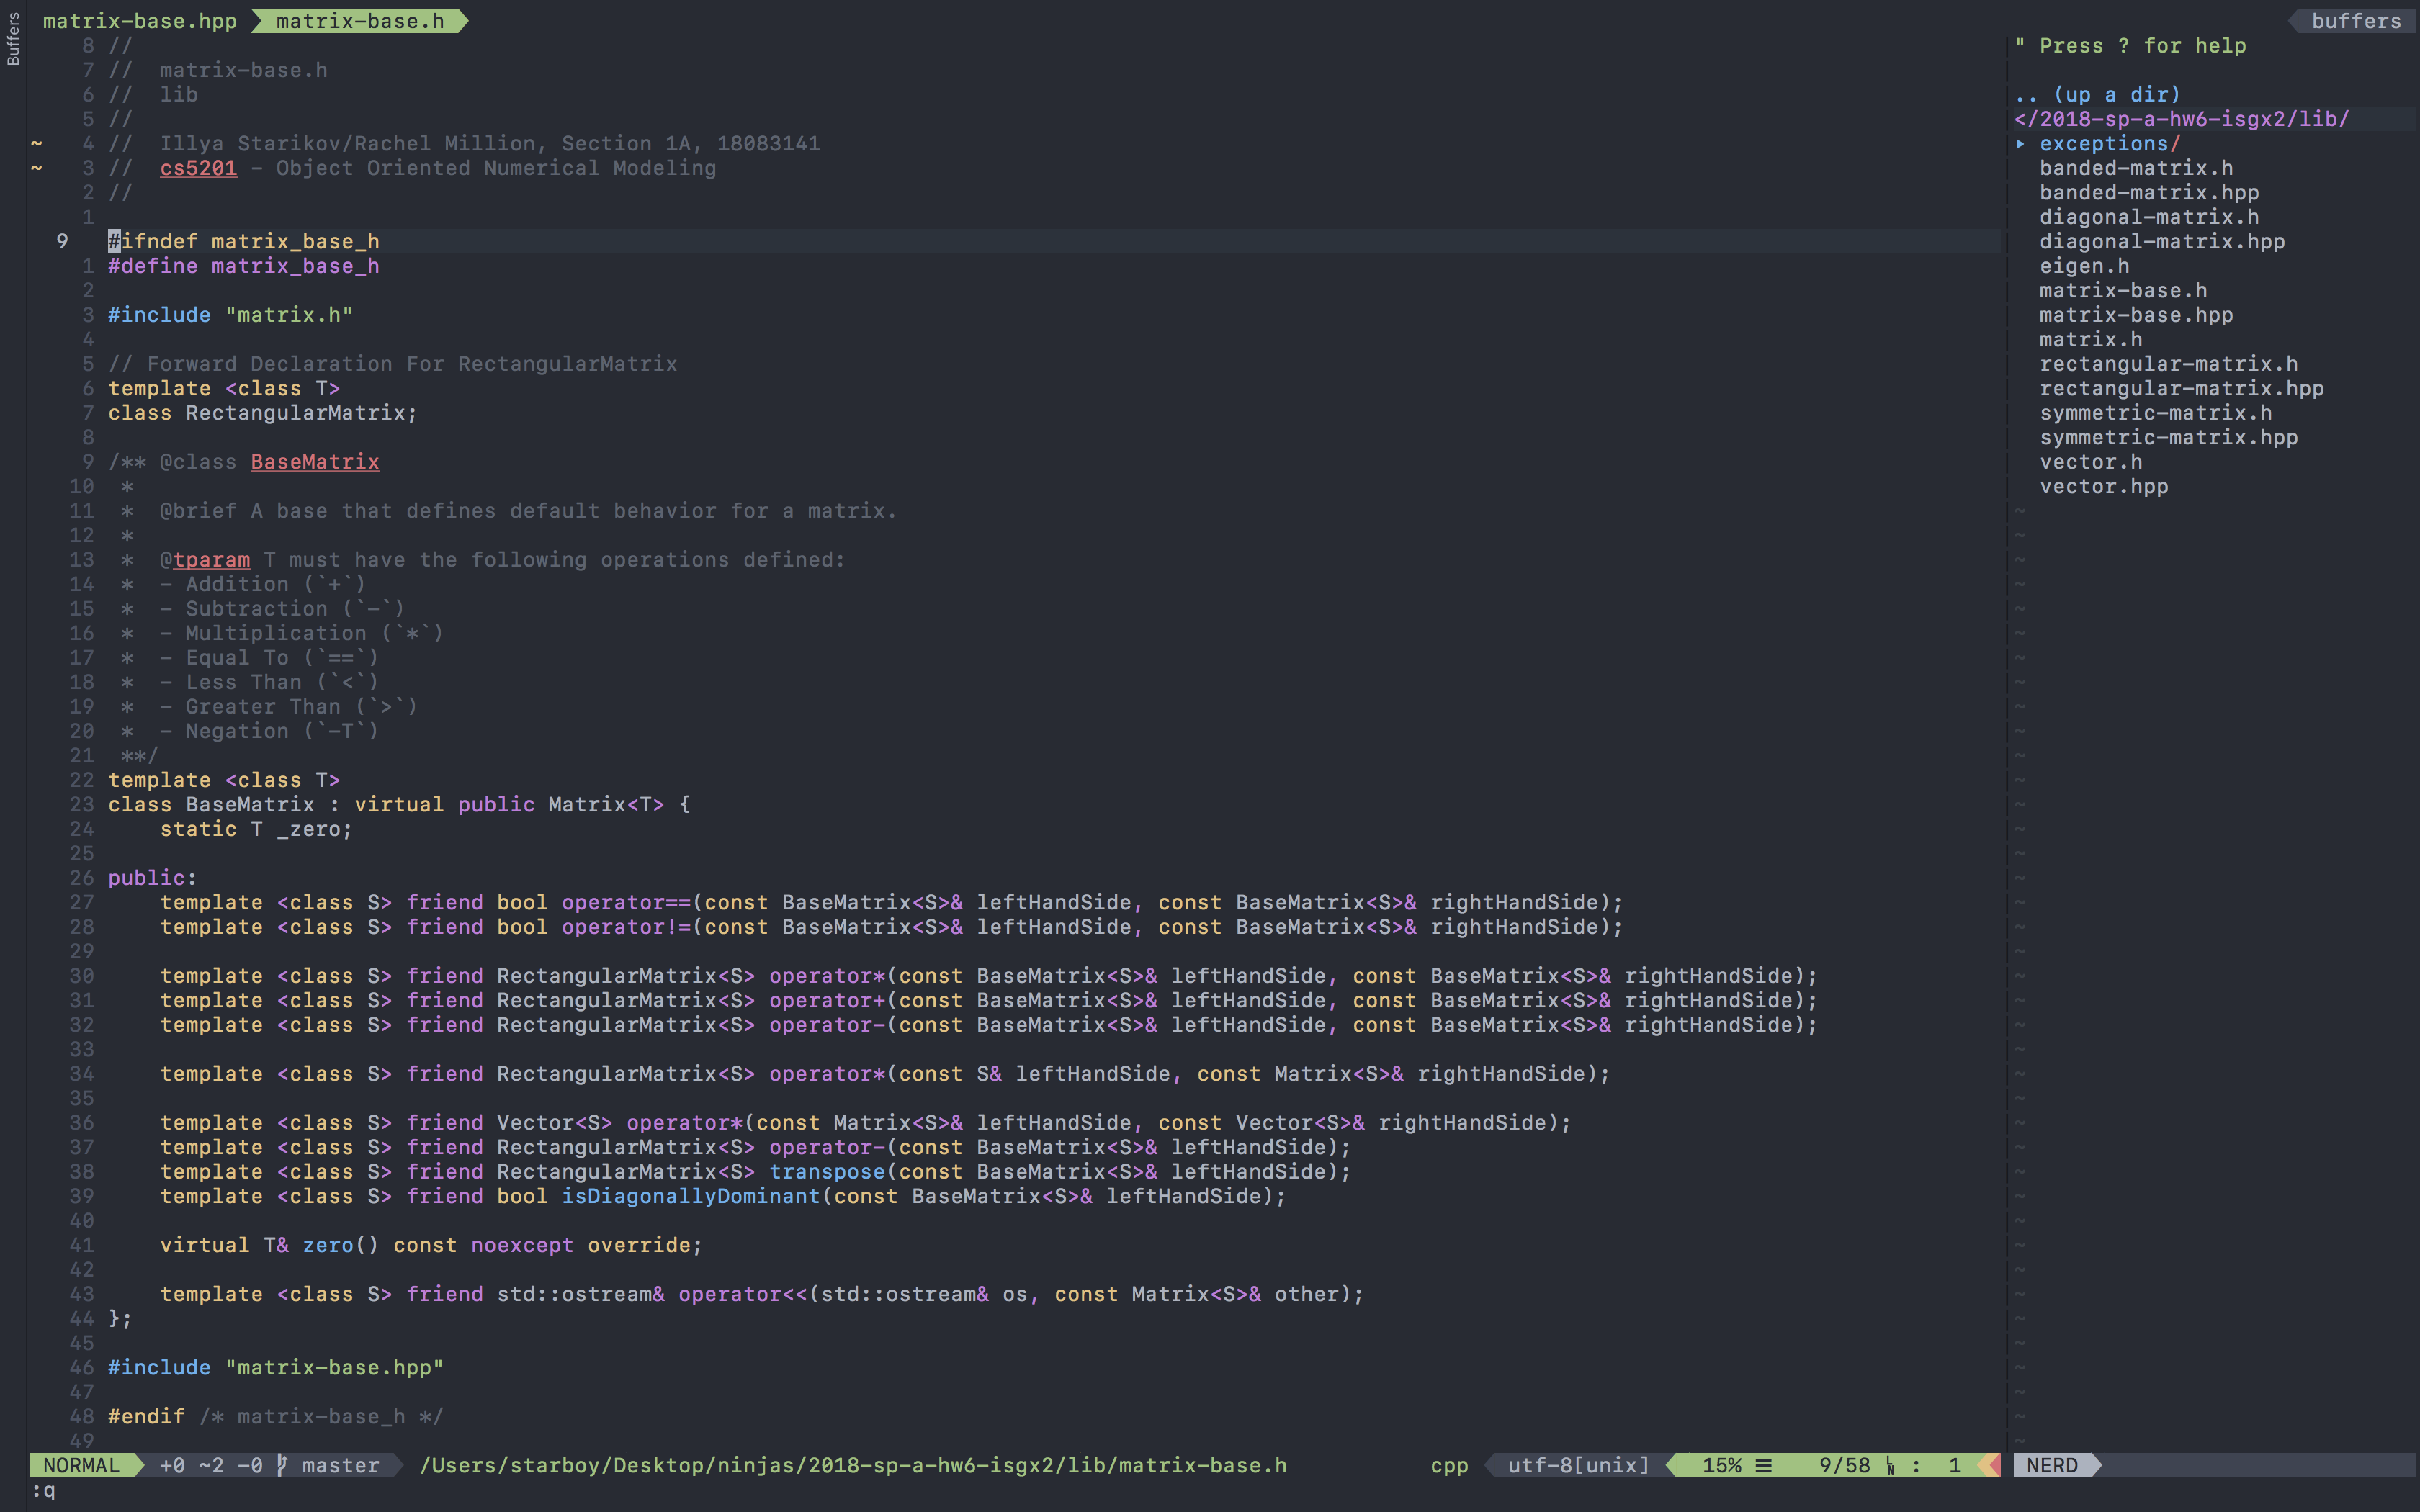
\includegraphics[width=\linewidth,cfbox=white 1pt 1pt]{assets/vim.png}
            \label{fig:vim}
        \end{figure}
    \end{frame}


    \begin{frame}
        \frametitle{Prior Knowledge}

        \begin{itemize}
            \item I've been using Vim since my freshmen year. However, I never worked with the advanced features of Vim, only the top level features.
            \item I knew that Vim had an expansive feature set, and I wanted to dive into that.
        \end{itemize}
    \end{frame}


    \begin{frame}
        \frametitle{Motivation}

        \begin{itemize}
            \item Upon graduation, I will likely be using Vim full time at my time at Garmin.
        \end{itemize}
    \end{frame}


    \begin{frame}
        \frametitle{Goals}

        \begin{itemize}
            \item To become more efficient at using Vim.
            \item To become familiar with the modern parts of Vim.
            \item To learn more of the keystrokes and shortcuts for Vim.
        \end{itemize}
    \end{frame}

    \begin{frame}
        \frametitle{Resources}

        \begin{itemize}
            \item A lot of the learning came from playing around with Vim. Anytime I found myself doing something repetitive, I simply tried to find a way to automate. Most of the time, there was a way.

            \item Book Resources (That I Actually Bought!):
                \begin{itemize}
                    \item \href{https://pragprog.com/book/modvim/modern-vim}{Modern Vim}
                    \item \href{https://pragprog.com/book/dnvim2/practical-vim-second-edition}{Practical Vim}
                \end{itemize}

            \item Online Resources:
                \begin{itemize}
                    \item \href{https://www.reddit.com/r/vim/}{The Vim Subreddit}, for everyday improvements or general knowledge on Vim.
                    \item \href{http://vimcasts.org}{VimCasts}, for when I want to get a deeper look into a subject.
                    \item \href{https://vim-adventures.com}{Vim Adventures}, a little game to help understand Vim through a text adventure.
                \end{itemize}
        \end{itemize}
    \end{frame}

    \begin{frame}
        \frametitle{Goal Accomplishment}

        \begin{itemize}
            \item I am much more fluent in using Vim, using shortcuts that significantly improve my workflow.
                \begin{itemize}
                    \item See attached videos for details.
                \end{itemize}

            \item I have also learned to use plugins, to do completions.
            \item I have also learned to use many of the different parts of Vim I was unfamiliar with, such as:
                \begin{itemize}
                    \item Buffers
                    \item Registers
                    \item Advanced Search
                    \item Tags
                \end{itemize}

                And a lot more!
        \end{itemize}
    \end{frame}

    \begin{frame}
        \frametitle{Side Note}

        \begin{figure}[H]
            \centering
            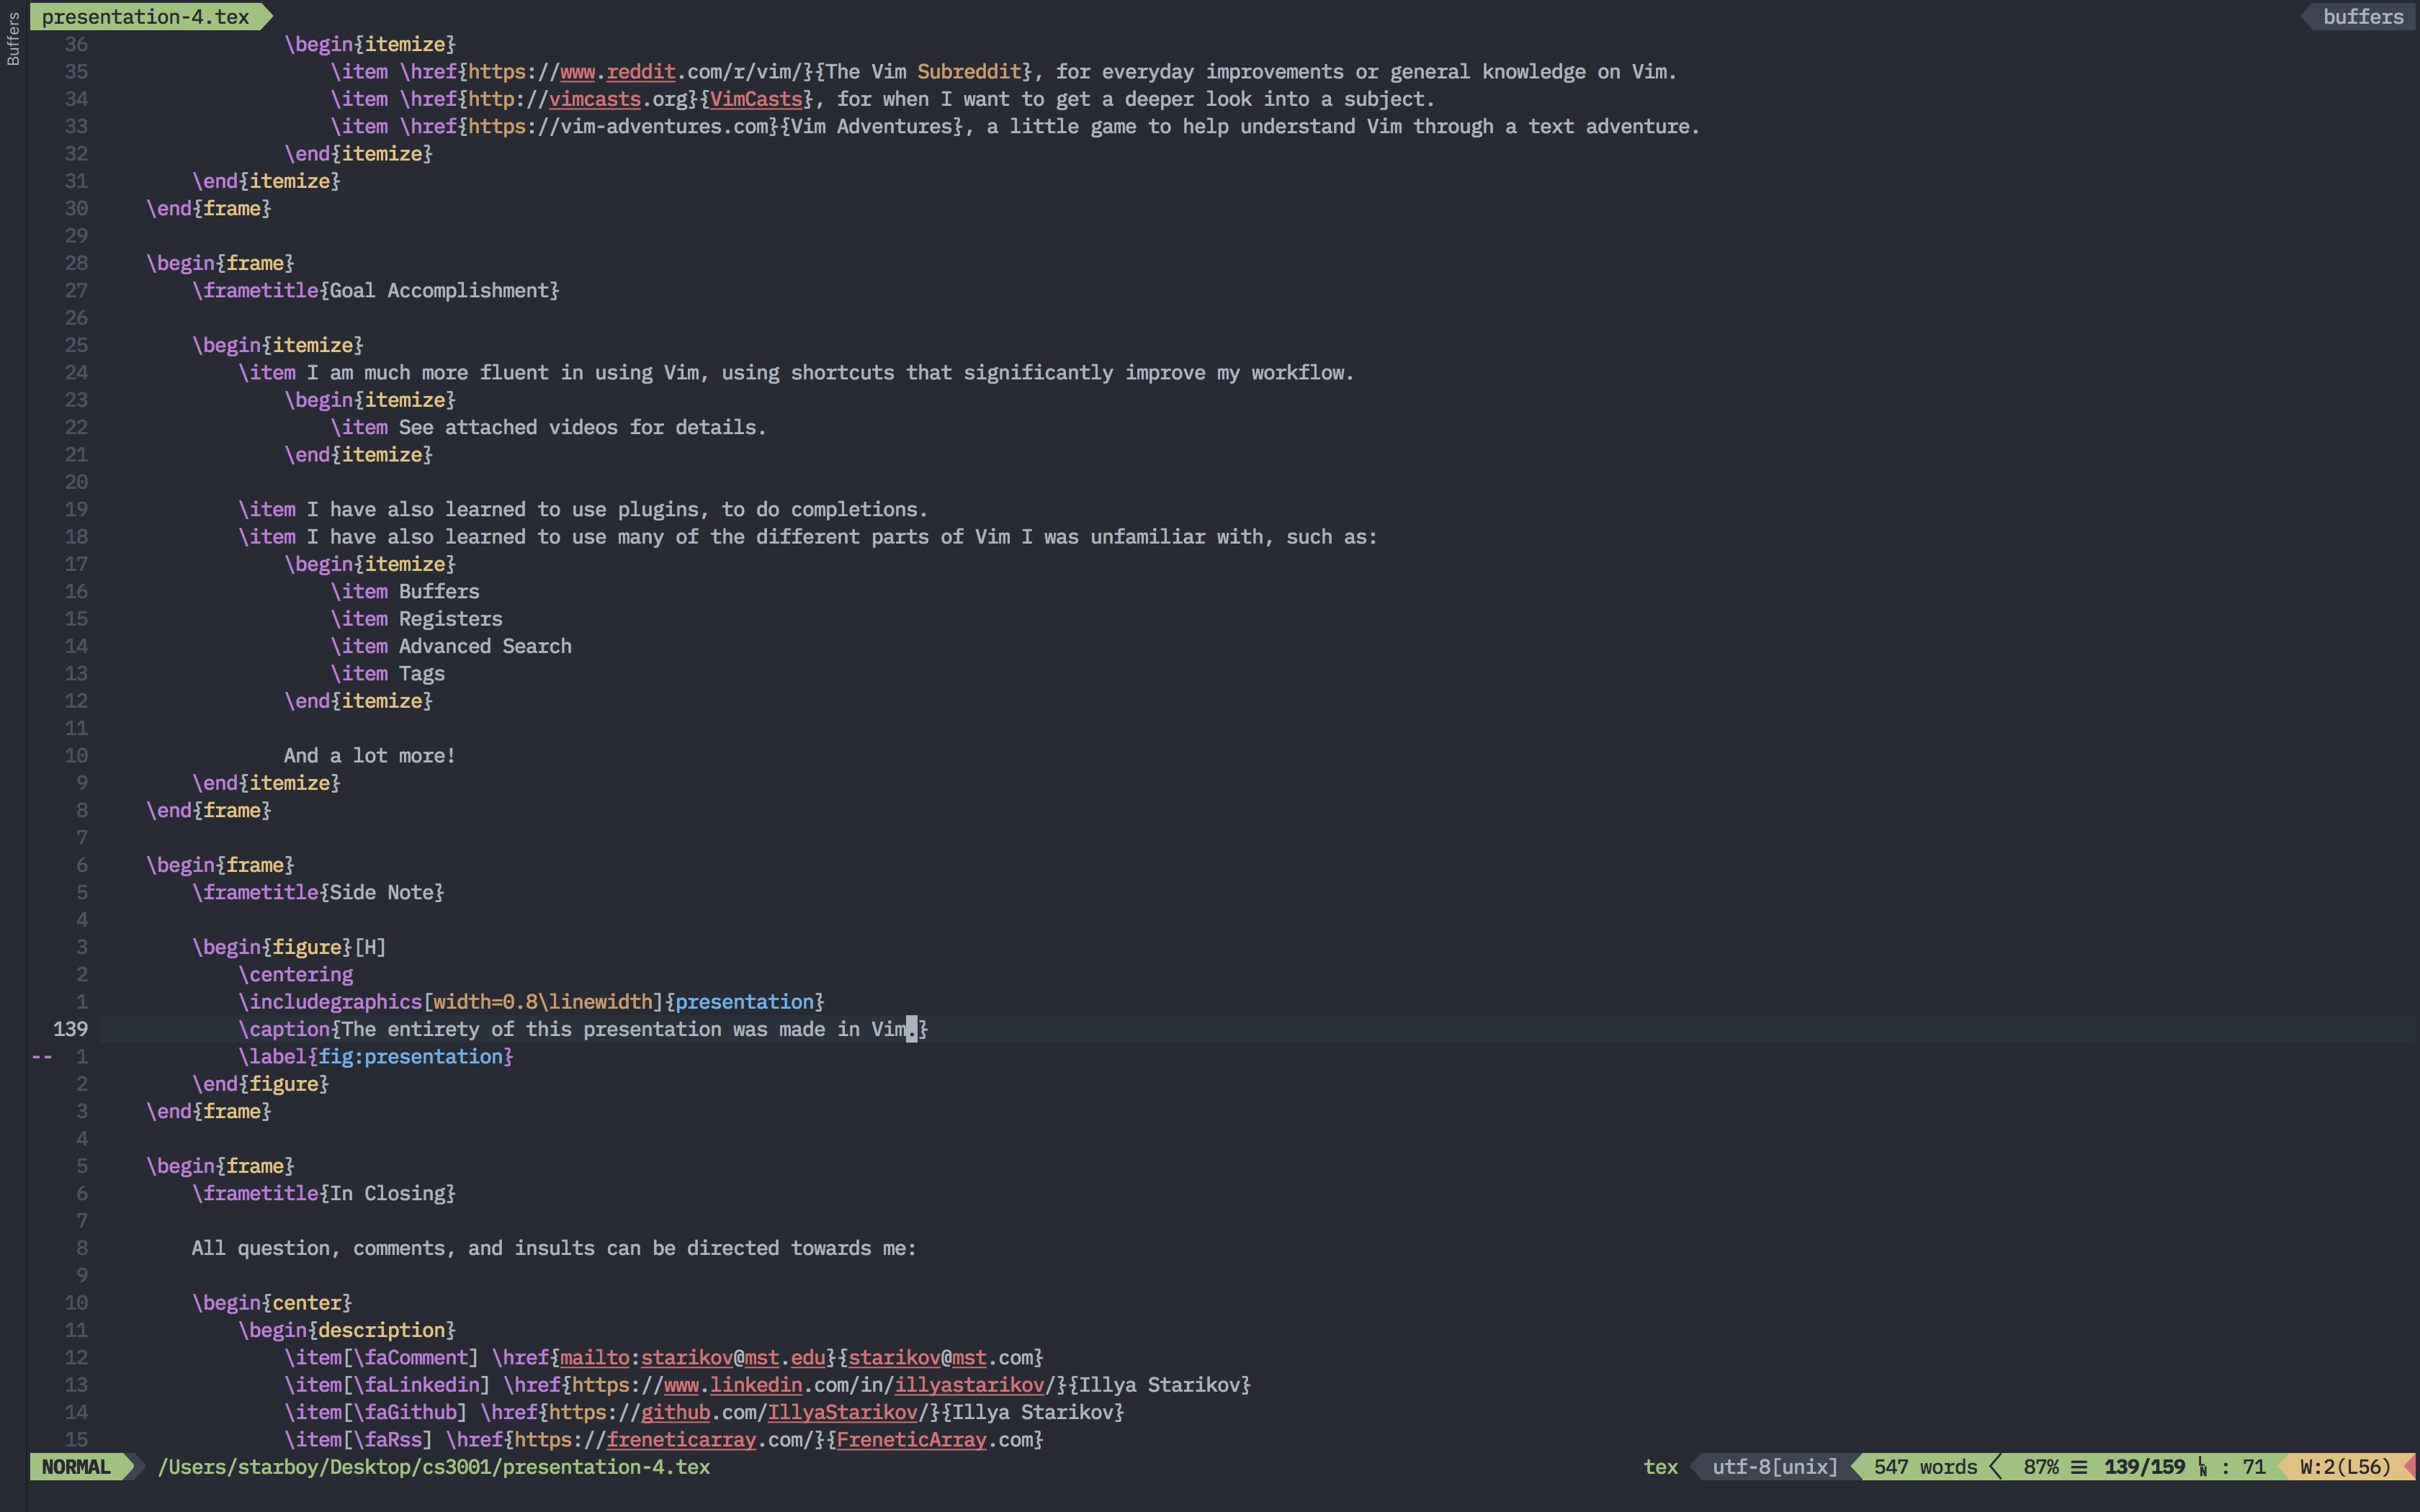
\includegraphics[width=0.95\linewidth]{assets/presentation.png}
            \caption{The entirety of this presentation was made in Vim.}
            \label{fig:presentation}
        \end{figure}
    \end{frame}

    \begin{frame}
        \frametitle{In Closing}

        All question, comments, and insults can be directed towards me:

        \begin{center}
            \begin{description}
                \item[\faComment] \href{mailto:starikov@mst.edu}{starikov@mst.com}
                \item[\faLinkedin] \href{https://www.linkedin.com/in/illyastarikov/}{Illya Starikov}
                \item[\faGithub] \href{https://github.com/IllyaStarikov/}{Illya Starikov}
                \item[\faRss] \href{https://freneticarray.com/}{FreneticArray.com}
            \end{description}
        \end{center}
    \end{frame}
\end{darkframes}
\end{document}
